\documentclass[10pt,a4paper,onecolumn,titlepage]{article}
\usepackage[utf8]{inputenc}
\usepackage[croatian]{babel}
\usepackage{amsmath}
\usepackage{amsfonts}
\usepackage{amssymb}
\usepackage{graphicx}
\usepackage{hyperref}
\usepackage{listings}
\usepackage{xcolor}

\lstdefinestyle{sharpc}{language=[Sharp]C, frame=lr, rulecolor=\color{blue!80!black}}
\title{Višekorisnička chat aplikacija u C\#-u}
\author{Antonio Kovačić\\Janko Marohnić\\Lana Arzon}

\begin{document}
\maketitle

\tableofcontents

\newpage

\section{Opis problema}

Potrebno je napraviti aplikaciju za gdje se ljudi mogu međusobno dopisivati
u realnom vremenu. Dvije ili više osoba se treba moći "naći na jednom mjestu",
i komunicirati zajedno putem tekstualnih poruka.

Kada se osoba prijavi u chat, treba upisati svoje korisničko ime, kojim će se
ta osoba identificirati. Ako je postoji druga osoba u istoj "sobi" koja već
ima željeno korisničko ime, osoba bi trebala izabrati drugo korisničko ime.
Nakon što je upisala korisničko ime, osoba mora moći vidjeti koji su sve drugi
korisnici trenutno prijavljeni u istu "sobu".

Kada osoba pošalje poruku u grupni chat (napiše teskt i stisne "enter"), svaka
druga osoba mora primiti tu istu poruku (i treba pisati od koga dolazi). Na taj
način svatko zna što su svi ostali rekli. I poruke moraju stizati redom kojim
su poslane.

Kada se osoba odjavi iz chata, ostalim osobama treba doći poruka da se ta
osoba odjavila iz chata.

\section{Implementacija}

\subsection{Server}

\subsubsection{Kreiranje}
Windows servis je program koji zapravo radi u pozadini dok je korisnik prijavljen na korisnički račun unutar Windows operativnog sustava. Podešavanjem
konfiguracija u \texttt{Command Promptu} Windows servis postaje aktivan. Samo kreiranje Windows servisa (detaljnim opisom što radi) se vrši kodiranjem u \textit{C\#}.
Najprije kreiramo novi projekt u \textit{C\#}, odabirući opciju Windows Service. Zatim
rekonstruiramo metodu $OnStart$ - dodajemo k\^{o}d za otvaranje (instanciranje)
kanala, registraciju objekata (dio tog koda \textit{C\#} doda automatski), itd. Zatim
se instalacija vrši na jednostavan način preko Visual Studia, odnosno \texttt{Command
Prompta}.
\lstset{style=sharpc}
\begin{lstlisting}[numbers=left, breaklines=true]
protected override void OnStart(string[] args) {
      BinaryServerFormatterSinkProvider provider = new BinaryServerFormatterSinkProvider(); 
      provider.TypeFilterLevel = System.Runtime.Serialization.Formatters.TypeFilterLevel.Full; 
      IDictionary props = new Hashtable(); props["port"] = 12345; //server ce slushati a portu 12345
      TcpChannel channel = new TcpChannel(props, null, provider); 
      ChannelServices.RegisterChannel(channel); //registriranje na kanal
      RemotingConfiguration.RegisterWellKnownServiceType(typeof(ChatServer), "Chat.ChatServer", WellKnownObjectMode.Singleton);//ime servera je "Chat.Chatserver"
    }

\end{lstlisting}
\subsubsection{Instaliranje}
Za postavljanje servisa smo napomenuli da ga moramo konfigurirati najprije
preko \texttt{Command Prompta}. Nakon prevođenja koda Windows servisa, dobivamo binarnu (izvršnu) datoteku Chat.exe. Najprije u \texttt{Command Promptu} trebamo otići u direktorij .NET Framework v. 4 naredbom:\\
\texttt{cd "C:$\backslash$Windows$\backslash$Microsoft.NET$\backslash$Framework64$\backslash$v4.0.30319"}\\
Potom naredbom:\\
\texttt{installutil "C:$\backslash$Ciljni\_ direktorij$\backslash$Chat$\backslash$bin$\backslash$Debug$\backslash$Chat.exe"}\\
instaliramo dani windows servis.
\subsubsection{Pokretanje}
Pokretanje servisa se vrši na sljedeći način: pokrenemo \texttt{Administrative tools}
preko \texttt{Control Panela} (ili preko \texttt{Search programs and files} na startnoj liniji Windowsa. Zatim odaberemo opciju \texttt{Services} u kojoj nađemo \texttt{ChatService}
(tako smo nazvali naš servis). Lijevim odabirom na opciju \texttt{Start} pokrećemo
dani servis.
\begin{figure}[!ht]
\begin{minipage}{\textwidth}
\centering
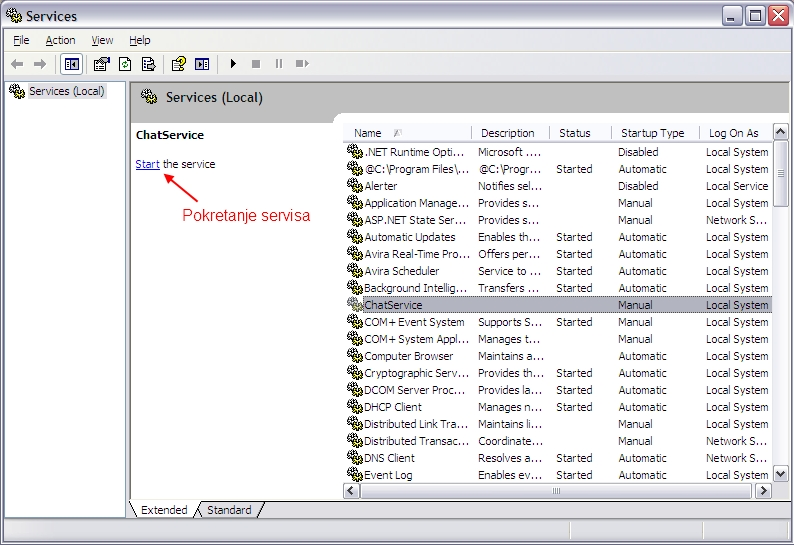
\includegraphics[width=\textwidth]{images/start_service.jpg}
\caption{Pokretanje servisa ChatService}
\end{minipage}
\end{figure}

\subsection{Klijent}

U klijentu nalazimo TCP kanal servisa, i spojimo se na server. Ako servis
nije upaljen, javljamo grešku.

Zatim ispisujemo poruku dobrodošlice, i vadimo sa servisa sve trenutno prijavljene
korisnike, i ispisujemo njihova korisnička imena novopridošlom korisniku. 

\begin{figure}[!ht]
\begin{minipage}{\textwidth}
\centering
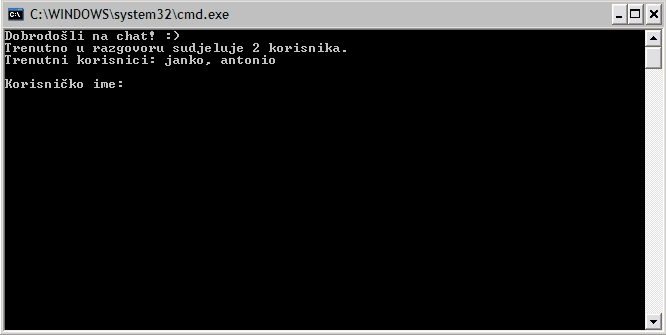
\includegraphics[width=\textwidth]{images/welcome.jpg}
\caption{Poruka dobrodošlice, broj prijavljenih korisnika i ispis njihovih korisničkih imena}
\end{minipage}
\end{figure}

Zatim ga tražimo da upiše svoje korisničko ime, s time da server provjerava postoji li
već korisničko ime, i u tom slučaju traži korisnika da upiše drugo korisničko ime.

\begin{figure}[!ht]
\begin{minipage}{\textwidth}
\centering
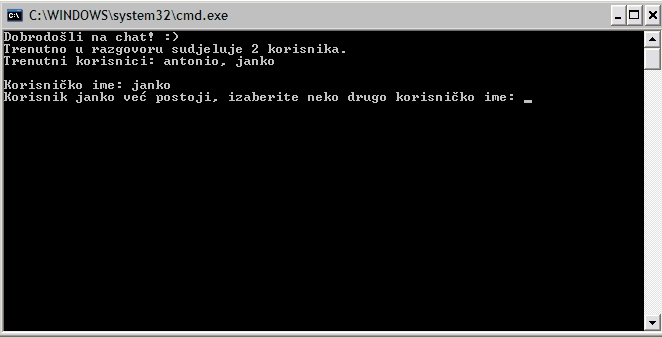
\includegraphics[width=\textwidth]{images/invalid_username.jpg}
\caption{Nemogućnost unosa već postojećeg korisničkog imena}
\end{minipage}
\end{figure}

Također, unos korisničkog imena je obavezan pa ako ga nismo unijeli, dobivamo upozorenje da to moramo učiniti.

\begin{figure}[!ht]
\begin{minipage}{\textwidth}
\centering
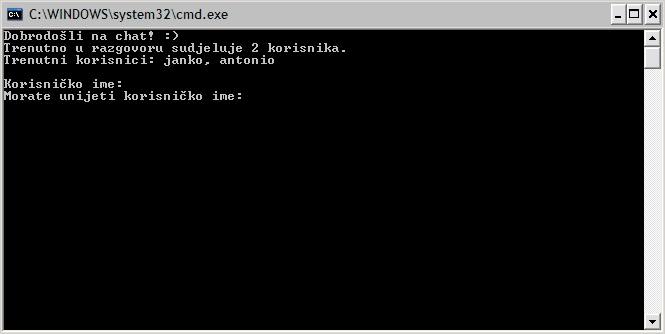
\includegraphics[width=\textwidth]{images/username_required.jpg}
\caption{Unos korisničkog imena je obavezan}
\end{minipage}
\end{figure}

Nakon prijave se svim korisnicima šalje obavijest da se novi korisnik prijavio
u chat, i korisnik se dodaje u servis.

\begin{figure}[!ht]
\begin{minipage}{\textwidth}
\centering
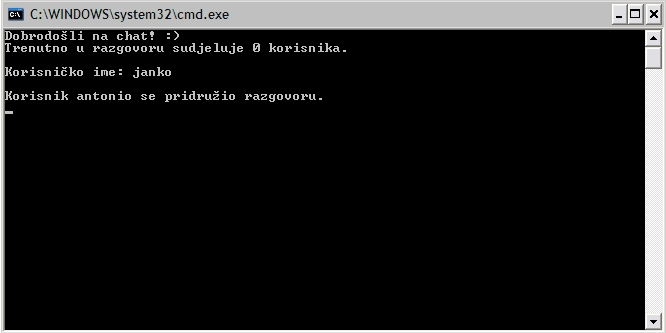
\includegraphics[width=\textwidth]{images/joining_notification.jpg}
\caption{Korisnik se pridružje razgovoru}
\end{minipage}
\end{figure}

Komunikacija se odvija na način da korisnik unese poruku koju zatim server prosljeđuje svim ostalim korisnicima koji su prijavljeni na chat.

\newpage

\begin{figure}[!ht]
\begin{minipage}{\textwidth}
\centering
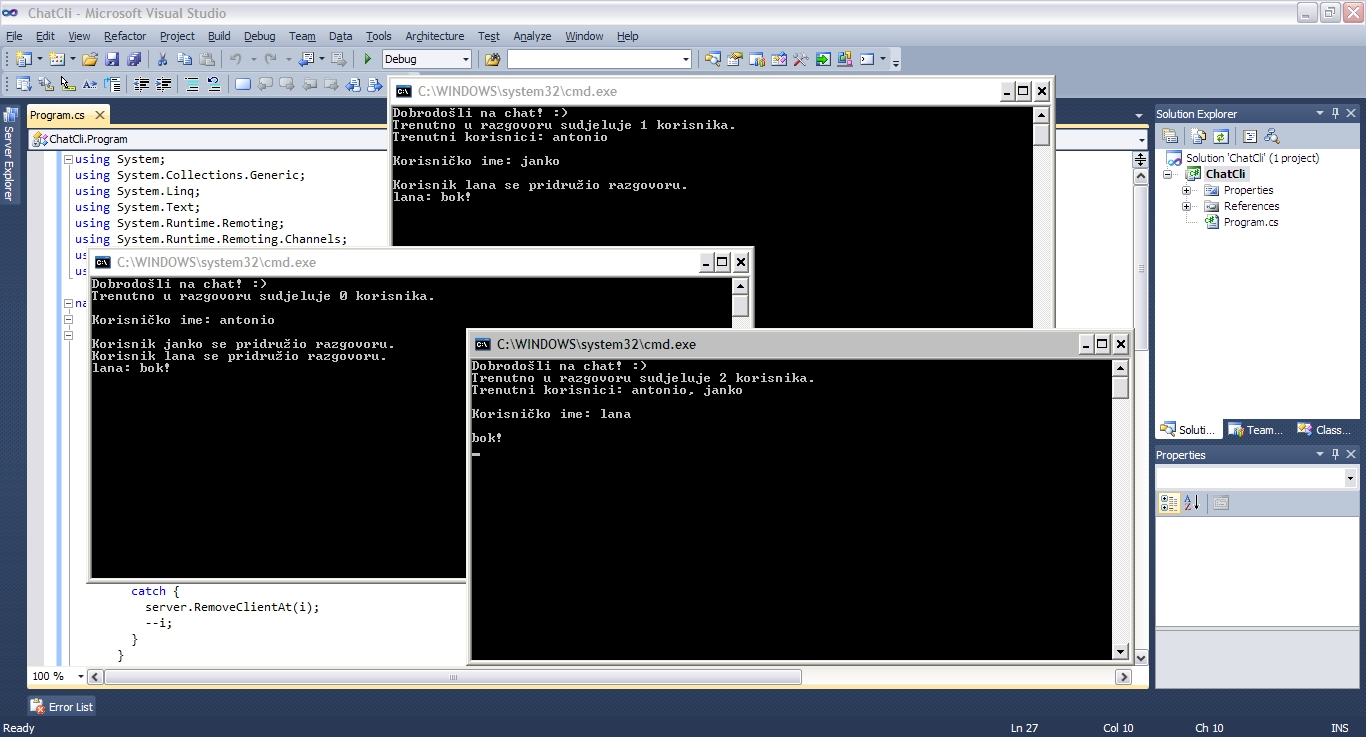
\includegraphics[width=\textwidth]{images/comunication.jpg}
\caption{Primjer jednostavne komumnikacije}
\end{minipage}
\end{figure}

Korisnik može u bilo kojem trenutku napustiti razgovor te nakon što to učini, svi ostali korisnici dobivaju obavijest o tome.

\begin{figure}[!ht]
\begin{minipage}{\textwidth}
\centering
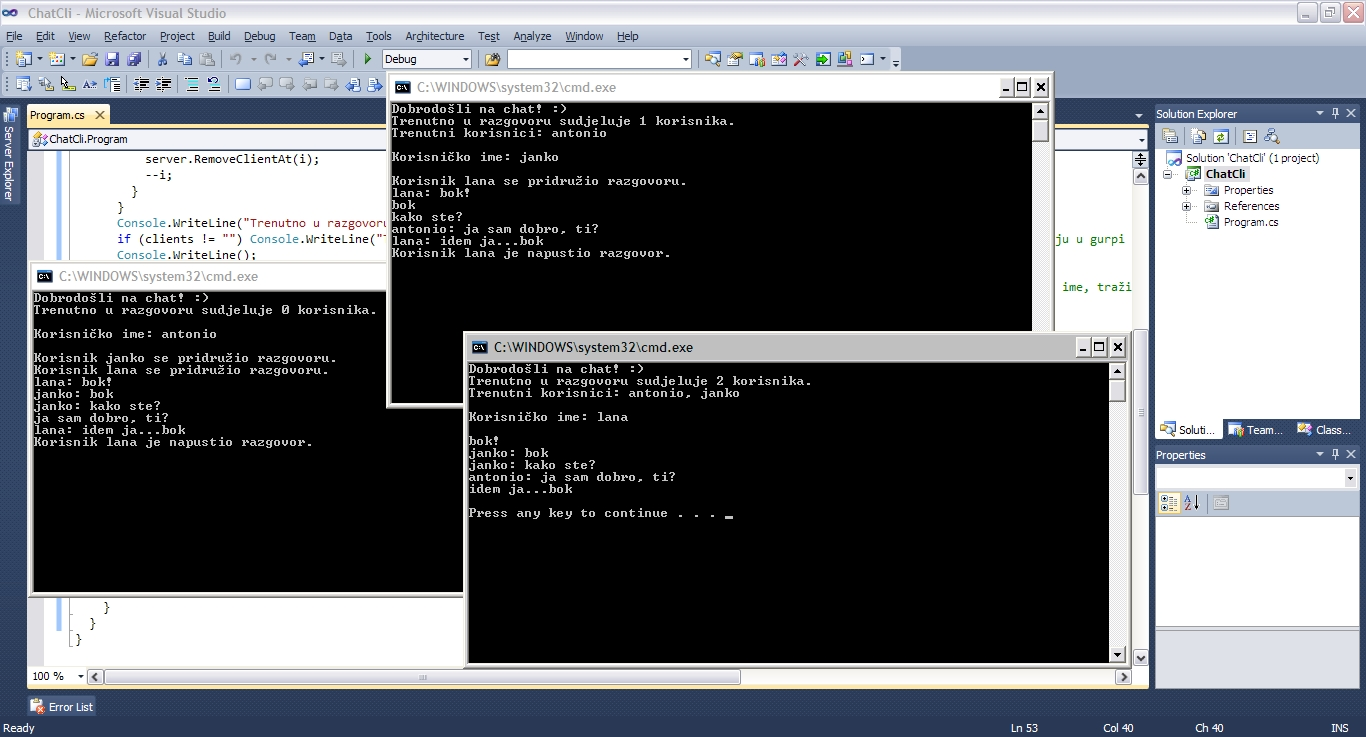
\includegraphics[width=\textwidth]{images/leaving_notification.jpg}
\caption{Korisnik napušta razgovor}
\end{minipage}
\end{figure}

\section{Rasprava}

Ova implementacija ima nekoliko prednosti. Jedna je da smo koristili Windowsove
servise za server, umjesto da smo implementirali svoj vlastiti. Na taj način
možemo biti sigurni da je taj server optimiziran i za veći broj korisnika.
Druga je što danas programeri uglavnom provode vrijeme u komandnoj liniji,
pa činjenica da je naša chat aplikacija napisana kao komandno-linijska aplikacija
pruža takvim korisnicima već poznato okruženje. Treća prednost je to što prestankom rada računala, prestane raditi i servis, pa nemamo problema sa eventualnim
cachiranjem koje bi druge implementacije mogle napraviti.

Neke mane naše implementacije su da, ukoliko korisnik zatvori prozor, naš servis
ne registrira da se korisnik odjavio (jer je zapravo došlo do iznimke, a naš
program trenutno ne obrađuje tu iznimku). Druga mana je da kada korisnik
piše poruku, a u isto mu vrijeme stigne poruka od nekog drugog korisnika,
zbog ograničenja komandne linije će mu pisanje vizualno prekinuti novopristigla
poruka. Korisnik još uvijek može dovršiti svoju poruku, i normalno je poslati,
samo mu se može učiniti da je došlo do greške.

\end{document}
